\section{Related Work}\label{sec:rw}

% \cc{TODO: ASPLOS reviewer suggestions~\cite{Yan2017}.}

% \cc{TODO: interesting recent work on Ocaml~\cite{Midtgaard2017}, jsfunfuzz, AFL, libFuzzer.}

The random generation of test cases is a well established approach to the compiler validation problem. Prior approaches are surveyed in~\cite{Kossatchev2005,Boujarwah1997} and empirically contrasted in~\cite{Chen2014a}. The main question of interest is in how to efficiently generate codes which trigger bugs. There are two main approaches: \emph{program generation}, in which inputs are synthesized from scratch, typically by stochastic enumeration of a grammar; and \emph{program mutation}, in which existing codes are modified and mutated so as to identify anomalous behavior.

\begin{figure}
	\centering %
	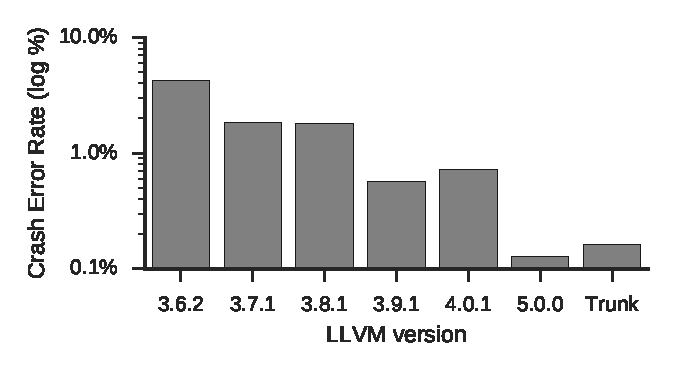
\includegraphics[width=.85\columnwidth]{build/img/clang-crashes}%
	\caption{%
		Crash rate of the Clang front-end of every LLVM release in the past 24 months compiling 75k DeepSmith kernels.
	}%
  \vspace{-0.8em}
	\label{fig:clangs} %
\end{figure}
\begin{table}
	\footnotesize %
	\centering %
	\begin{tabular}{r|ccccccc}
\toprule
{} & 3.6.2 & 3.7.1 & 3.8.1 & 3.9.1 & 4.0.1 & 5.0.0 & Trunk \\
\midrule
Assertion 1 &  2962 &  1327 &  1332 &   414 &   523 &    83 &    97 \\
Assertion 2 &       &     1 &     1 &       &       &       &       \\
Assertion 3 &       &       &       &       &       &       &     1 \\
Assertion 4 &       &       &       &       &       &       &     2 \\
Assertion 5 &   147 &       &       &       &       &       &       \\
Assertion 6 &     1 &       &       &       &       &       &       \\
Assertion 7 &       &       &       &     1 &     1 &       &       \\
Unreachable &    86 &    42 &    14 &    14 &    18 &    13 &    21 \\
\bottomrule
\end{tabular}

	\caption{%
		The number of DeepSmith programs which trigger distinct Clang front-end assertions, and the number of programs which trigger unreachables.%
	}
  \vspace{-3.1em}
	\label{tab:clangs}
\end{table}

\paragraph{Program Generation}

In the foundational work on differential testing for compilers, McKeeman \emph{et al.\ }present generators capable of enumerating programs of a range of qualities, from random ASCII sequences to C model conforming programs~\cite{McKeeman1998}. Subsequent works have presented increasingly complex generators which improve on the prior in some metric of interest, generally expressiveness or probability of correctness. CSmith~\cite{Yang2011} is a widely known and effective generator which enumerates programs by pairing infrequently combined language features. In doing so, it produces correct programs with clearly defined behavior but very unlikely functionality, increasing the chances of triggering a bug. Achieving this required extensive engineering work, most of it not portable across languages, and ignoring some language features. Subsequent generators influenced by CSmith, like Orange3~\cite{Nagai2013}, focus on features and bug types beyond the scope of CSmith, arithmetic bugs in the case of Orange3.

\paragraph{Program Mutation}

Equivalence Modulo Inputs (EMI) testing~\cite{Le2013a,Sun2016a} follows a different approach to test case generation. Starting with existing code, it inserts or deletes statements that will not be executed, so functionality should remain the same. If it is affected, it is due to a compiler bug. While a powerful technique able to find hard to detect bugs, it relies on having a very large number of programs to mutate. As such, it still requires an external code generator. Similarly to CSmith, EMI favors very long test programs. LangFuzz~\cite{Holler2012} also uses mutation but does this by inserting code segments which have previously exposed bugs. This increases the chances of discovering vulnerabilities in scripting language engines.
% \cc{TODO: Expand discussion}
Skeletal program enumeration~\cite{Zhang2017a} again works by transforming existing code. It identifies algorithmic patterns in short pieces of code and enumerates all the possible permutations of variable usage.
% \cc{TODO: no testing of invalid inputs, unclear if scales to complex programs.}

\paragraph{Test case Reduction} With both generation and mutation based approaches, bug-exposing programs can be unnecessarily long. While 80\% of the test cases related to GCC and LLVM bugs are 45 lines~\cite{Sun2016} or less, CSmith/EMI output tends to be thousands of lines long. Most this code is not related to the bug and has to be removed for compiler engineers to understand the source of the problem. To that end test case reduction techniques~\cite{Regehr2012a,Pflanzer2016,Herfert} have been developed to bring the code down to manageable lengths. These techniques are very slow, potentially taking several hours to reduce a single test case. Automated reducers also require extensive engineering effort, applying analyses at every stage of the iterative reduction process so as not to obscure the bug-exposing property of interest. Another common problem is prioritizing the most important bugs out of the hundreds or thousands discovered. This \emph{fuzz taming problem} is addressed in~\cite{Chen2013}, in which a distance metric is used to rank test cases such that diverse, interesting test cases are highly ranked. % \cc{TODO: Our approach complements EMI}

Compared to all these, our fuzzing approach is low cost, easy to develop, portable, capable of detecting a wide range of errors, and focusing by design on bugs that are more likely to be encountered in a production scenario.


%CSmith~\cite{Yang2011} and CLSmith~\cite{Lidbury2015a}. Same testing methodology, but very different design goals to our work. The explore the space of \emph{unlikely} programs, by pairing infrequently combined language features. Because Csmith programs are free form undefined behavior, there is only a single interpretation. This allows oracle-less differential testing across compilers, using a voting heuristic to identify erroneous compiler outputs. The ``shape'' of programs generated by Csmith is expert driven. The shape of programs generated by DeepSmith is data driven. The 80 probabilities which control Csmith program generation are extensively hand tuned to produce programs which ``look right''. Our data driven approach does not require this. In fact, our approach is portable across changing usage of a programming language.

%The functionality of Csmith is also expert driven. Every language feature supported by Csmith must be laboriously hand crafted, and results in a very complex system of over 40,000 lines of C++ code (which still omits many language features used in real programs, like heap allocation). The language features supported by DeepSmith is bound only by those which have been used on GitHub. DeepSmith has a non-zero probability of generating programs using every language feature found on GitHub. We reason that if a language feature remains unused in the entirety of code on GitHub, then it is reasonable to assume that it is not a feature worth testing. Both Csmith and CLsmith use unrealistic safe-math macros to wrap arithmetic operations. We do not.


% Increasing complexity of generations: RandProg to CSmith. Then EMI testing, and SPE.

%The \emph{fuzz taming problem} is addressed in~\cite{Chen2013}, in which a distance metric is used to rank test cases such that diverse, interesting test cases are highly ranked.

%\emph{LangFuzz} attempts a similar approach of learning to generate test cases from real code~\cite{Holler2012}. For LangFuzz, the input programs are codes known to have previously exposed bugs.

%Empirical comparison of compiler testing techniques~\cite{Chen2014a}

%\cc{is it wise to draw attention to this?} If the output of a program depends on undefined or unspecified behavior, then comparing outputs across compilers is meaningless. Prior works have formulated random program generation so as to minimize or eradicate the possibility of undefined and unspecified behavior~\cite{Yang2011c,Le2013a,Le2015}, at the expense of expressiveness. Recently, work in Skeletal Program Enumeration~\cite{Zhang2017a} has relied on handchecking of C programs and tools such as CompCert~\cite{Leroy2013} and UBsan to detect false-positives. Since DeepSmith programs are not guaranteed to be free from undefined behaviors, and we can only determine if a program is well-formed empirically, additional filtering of test cases is required to prevent false-positives.

%Analysis of bugs in GCC and LLVM finds 80\% of test cases to be 45 lines~\cite{Sun2016}.

%\cc{TODO}~\cite{Godefroid2008a,Le2015,Sun2016a}~\cite{Kossatchev2005}.

%\cc{TODO:} Directed EMI testing~\cite{Le2015}.

%\cc{TODO: finding arithmetic bugs which CSmith cannot~\cite{Nagai2013}}

%``As a matter of implementation quality, a compiler vendor will usually fix a segmentation fault or similar problem even if the crash-inducing test case, for example, uses a variable without initialization.''~\cite{Regehr2012a}

%Skeletal program enumeration~\cite{Zhang2016a}. By enumerating entire program space, provides bounded guarantees of compiler correctness. Same shortcoming as CSmith (well formed programs only). No OpenCL implementation. Probably would take a lot of development effort. \cc{More investigation required.}

%Both tools require test case reduction (\cite{Regehr2012a} and~\cite{Pflanzer2016}, respectively). Work in test case reduction~\cite{Regehr2012a} reduced Csmith program sizes by 74--594$\times$ while preserving the bug exposing behavior. They median reduced CSmith program size they found was only 20 lines (0.5KB).

%\cc{TODO:}

%EMI testing~\cite{Le2013a}, Skeletal Program enumeration~\cite{Zhang2017a}.

%Fuzzing with code fragments~\cite{Holler2012}.

%A mutation-based approach for the Java Virtual Machine is demonstrated in~\cite{Chena}.

%TODO~\cite{White2016},~\cite{Sheridan2007}.

%Grammar-base whitebox testing~\cite{Godefroid2008a}.

%Our unique contribution is a low cost method for fuzzing, capable of detecting a wide range of errors, and matching that of human expectation (small, plausible test cases).


%HJL - Removing - \paragraph{GPU Testing} \pp{Do we really need this?} GPU Concurrency --- Small \emph{litmus tests}~\cite{Alglave2015}.
%GPUVerify~\cite{Bardsley2014}.

\paragraph{Machine Learning} In software testing,
machine learning has been successfully applied before on areas such as improving bug finding static analyzers~\cite{Heo2017,Koc2017}, repairing programs~\cite{Koukoutos2017a,White}, prioritizing test programs~\cite{Chen2017}, identifying buffer overruns~\cite{Choi2016}, and processing bug reports~\cite{Lam2016,Huo2016}. A proof-of-concept implementation of machine learning for input fuzzing is presented in~\cite{Godefroid2017}, although no bugs are found. % TODO: More on this?

\begin{table}
	\footnotesize %
	\centering %
	\begin{tabular}{rc|ccc}
\toprule
  \textbf{Compiler} & $\pm$ & \textbf{Silent Crashes} & \textbf{Assertion 1} & \textbf{Assertion 2}\\
\midrule
  \multirow{ 2}{*}{solc} & $-$ & 204 & 1 & \\
                         & $+$ & 204 & 1 & \\
  \hline
  \multirow{ 2}{*}{solc-js} & $-$ & 3628 & 1 & 1\\
                         & $+$ & 908 & 1 & 1\\
\bottomrule
\end{tabular}
	\caption{%
		% Results from 12 hours of testing Solidity compilers using DeepSmith.
		The number of DeepSmith programs that trigger Solidity compiler crashes from 12 hours of testing.%
     \vspace{-1em}
	}
   \vspace{-2em}
	\label{tab:solidity}
\end{table}

% \cite{Yan2017}

Deep Learning is a nascent field that is responsible for a multitude of breakthroughs in modeling rich, hierarchical datasets. The major milestones are reviewed in~\cite{Wang2017}, and methods in~\cite{Schmidhuber2014}. There is an increasing interest in mining source code repositories at large scale~\cite{Allamanis2017a}.
% \cc{Using machine learning to inductive program synthesis~\cite{Parisotto2016,Balog2017}.}
Previous studies have involved data mining of GitHub to analyze software engineering practices~\cite{Wu2014,Guzman2014,Baishakhi2014a,Vasilescu2015}, for example code generation~\cite{Zhang2015a}, comment generation~\cite{Wong2013}, and code completion~\cite{Raychev2014}.
% \cc{Creating compilable code snippets mined from StackOverflow~\cite{Terragni2016}}.
To the best of our knowledge, no work so far has succeeded in finding compiler bugs by exploiting mined source code for test case generation. Ours is the first to do so.
